\chapter{Úvod do teórie strojového učenia}

V oblasti teórie strojového učenia sa zaoberáme učením; formalizujeme ho,
navrhujeme rôzne algoritmy schopné tohto učenia, analyzujeme ako rýchlo
sa tieto algoritmy učia, ... Čo to ale vlastne je to ``učenie'', a ako sa
nad týmto konceptom dá zamýšľať?

Začnime tým, že si vybavíme, čo všetko sa nám spája s učením. Napríklad
učenie sa na skúšky, ktoré pre niektorých vyzerá tak, že sa snažia si
zapamätať všetkých $80$ strán skrípt naspamäť. Alebo keď sa snažíme
naučiť novú skladbu na klavíri: hráme ju znova a znova, až kým v tom
nie sme dobrí. Alebo trénovanie na dôležitý zápas vo futbale, ...

Vidíme teda, že učenie je zložitý koncept. Konkrétne detaily toho, ako
presne sa učíme (resp. prečo to funguje), sú známe málo ľuďom. Avšak
vidíme, že jednotlivé ``učenia'' mali niečo spoločné: nejaká aktivita
sa opakovala veľakrát, a čím viackrát sa zopakovala, tým lepší bol
výkon. Zároveň ale nechceme, aby sa zakaždým odohralo to isté; nová
skúsenosť je dôležitou súčasťou učenia.

Ak by sme len tak vychrlili nejakú definíciu, ktorá nám príde rozumná,
riskujeme, že nebude ``sedieť s našou intuíciou'', alebo nebude dostatočne
všeobecná. Kvôli tejto zložitosti teda namiesto toho, aby sme zachytili
``učenie'' v jednej definícii, študujeme veľa rôznych modelov učenia,
ktoré sú aplikovateľné v rôznych kontextoch. Pod ``modelom'' rozumieme
akúsi hračku, zjednodušený mentálny obraz, s ktorým sa jednoducho pracuje
a zároveň ``sedí s našou intuíciou''. Takto síce nijak neručíme, že pokrývame
``všetko učenie''; čím viac viet a teorém v rôznych modeloch ale dokážeme,
tým lepší budeme mať obraz o tom, čo to učenie je.

My sa v týchto skriptách budeme zaoberať hlavne oblasťou \emph{učenia s
učiteľom}. Uvedieme hlavný model (tzv. \emph{statistical learning framework}),
s ktorým budeme pracovať, a v prípade potreby rozširovať/dolaďovať.




\section{Model}

Predstavme si, že chceme vedieť na základe nejakých vstupných dát (ktoré
budeme spravidla označovať $x$) predpovedať výstupné dáta (označované $y$).
Napríklad chceme na základe rozlohy bytu vedieť predpovedať jeho cenu.
Alebo vedieť z obrázku (vo formáte $32 \times 32$ čiernobielych pixelov)
povedať, či sa v ňom nachádza mačka alebo nie.

Snažíme sa teda zachytiť nejaký vzťah medzi dátami $x$ a $y$. To, akým
spôsobom to budeme robiť, je nasledovné: nejakým procesom $P$ získame $t$
\emph{trénovacích príkladov} $(x_1, y_1), \ldots, (x_t, y_t)$. Na základe
týchto príkladov budeme chcieť navrhnút nejakú funkciu $h$, ktorá bude
vedieť podľa vstupu $x$ predpovedať výstup $y$ s dostatočnou presnosťou.

Prirodzený spôsob, akým môžeme merať úspešnosť funkcie $h$, je podľa
toho, ako sa jej darí na našich $t$ príkladoch. Prístupu, kde hľadáme
funkciu, ktorej sa čo najlepšie darí na trénovacích príkladoch, hovoríme
\emph{empirical risk minimization} (skrátene ERM). Dobrá funkcia $h$ ale
bude schopná aj \emph{generalizovať}: bude sa jej dariť na ďalších
dátach, ktoré vieme získať tým istým procesom $P$.

Schopnosť generalizácie je jednou z najdôležitejších vlastností, ktoré
od trénovania pomocou techník strojového učenia požadujeme. Predstavme si,
že by sme funkciu $h$ zostrojili tak, že si ``zapamätáme'' všetky trénovacie
príklady: ak je na vstupe $x$, ktoré bolo medzi trénovacími príkladmi,
vrátime príslušné $y$. Takáto funkcia $h$ má zrejme nulovú chybu na
trénovacích príkladoch (pokiaľ pre jedno $x$ existuje vždy len
jedno správne $y$), ale mimo nich sa jej vôbec nebude dariť.

Vidíme teda, že ERM vo svojej holej podstate nefunguje. Problém je v tom,
že neobmedzujeme to, aké funkcie považujeme sa ``kandidátov'': nič
nezaručuje, že informácia z trénovacích príkladov sa prenesie aj na
ostatné príklady. Obmedzíme teda množinu funkcii, ktoré uvažujeme,
na nejakú užšiu skupinu, ktorú nazveme \emph{množina hypotéz}.

Napríklad si predstavme, že hľadáme funkciu $f : \R \to \R$ a dostali
sme trénovacie príklady $(0, 0)$ a $(1, 1)$. Ak o probléme nič ďalšie
nevieme, tak nevieme povedať nič o tom, ako sa bude $f$ správať pre
$x \not\in \{0, 1\}$. Ak ale vieme, že hľadáme neklesajúcu funkciu
s oborom hodnôt $\{0, 1\}$, tak vieme, že $f(x) = 0$ pre $x \leq 0$,
$f(x) = 1$ pre $x \geq 1$, a niekde v intervale $(0, 1)$ sa to ``láme''.

Tým, že sme obmedzili množinu hypotéz, sme v podstate zaviedli
\emph{inductive bias}: predpoklady, ktoré využívame na to, aby
sme odvodili výsledky aj na tých vstupoch, ktoré sme ešte nevideli.




\section{Definície a označenia}

Množinu všetkých vstupov označíme $X$, niekedy jej budeme hovoriť aj
\emph{množina inštancii}. Množinu všetkých výstupov označíme $Y$.

Množinu všetkých trénovacích príkladov budeme volať \emph{trénovacia
množina}, označíme ju $T$. (Z matematického hľadiska to ale nie je
množina, skôr multimnožina, kedže jedna dvojica $(x, y)$ sa medzi
trénovacími príkladmi môže vyskytovať viackrát. Pre jednoduchosť to
ale budeme nazývať množinou.) Počet trénovacích príkladov označíme $t$.

Proces, ktorým získavame dáta $(x, y)$, vieme formalizovať ako
pravdepodobnostné rozdelenie $P$ nad priestorom $X \times Y$, ktoré
každému možnému pozorovaniu priradí nejakú pravdepodobnosť (resp. hustotu
pravdepodobnosti v prípade spojitého rozdelenia). Trénovacie
príklady získame ako $t$ nezávislých vzoriek z rozdelenia $P$.

Postup, ktorým zostrojíme funkciu $h$, vieme formalizovať ako algoritmus,
ktorý na vstupe dostane niekoľko trénovacích príkladov
$(x_1, y_1), \ldots, (x_t, y_t)$, a na výstupe vráti funkciu $h : X \to Y$,
ktorú budeme volať \emph{hypotéza}. Množinu hypotéz označíme $H$.

V tejto kapitole sa nebudeme zaoberať výpočtovou stránkou strojového
učenia, takže od detailov ako časová zložitosť, spôsob hľadania
optimálneho riešenia a pod. abstrahujeme.



\subsection{Meranie chyby hypotézy}

Ako vyjadriť mieru toho, že sa hypotéze ``dobre darí''? Spravíme tak
pomocou \emph{chybovej funkcie} $\err : Y \times Y \to \R^+_0$,
ktorej význam je nasledovný: $\err(y, y')$ vyjadruje, ako veľmi
sa od seba líšia výstupy $y$ a $y'$.

\emph{Chyba na jednom príklade.} Keď dostaneme nejaký príklad $(x, y)$,
vieme zmerať, ako veľmi sa naša hypotéza $h$ na tomto vstupe pomýlila,
ako $\err(h(x), y)$.

\emph{Očakávaná testovacia chyba hypotézy (OTeChHyp).} Celkovú chybu našej
hypotézy potom vieme zmerať ako očakávanú chybu na náhodne vybranom
príklade z rozdelenia $P$. Túto chybu budeme označovať $\Err$,
a vypočítame ju nasledovne:
$$\Err(h, P) = \E_{(x, y) \sim P} \left[ \err(h(x), y) \right].$$
Častokrát ale bude rozdelenie $P$ jasné z kontextu, v takom prípade
budeme skrátene písať $\Err(h)$.

\emph{Trénovacia chyba.} Niekedy nás bude zaujímať ale aj chyba,
ktorú hypotéza nadobúda na trénovacej množine. Budeme ju tiež
označovať $\Err$, a vypočítame ju nasledovne:
$$\Err(h, T) = \E_{(x, y) \in T} \left[ \err(h(x), y) \right] = \frac{1}{t} \cdot \sum_{i=1}^t \err(h(x_i), y_i).$$
Tento zápis sa dá chápať aj tak, že trénovaciu množinu interpretujeme
ako pravdepodobnostné rozdelenie, pričom pravdepodobnosť každého príkladu
je úmerná tomu, koľkokrát sa v množine vyskytuje. Niekedy túto chybu
budeme zapisovať aj $\Err_T(h)$.



\subsection{Meranie chyby algoritmu}

Hypotéza je iba výstupom trénovacieho algoritmu, a závisí od toho, akú
konkrétnu trénovaciu množinu dostaneme a od prípadnej náhodnosti
samotného algoritmu. Ak by sme chceli porovnať dve rôzne algoritmy,
na úrovni výstupných hypotéz to nevieme spraviť: pre jednu trénovaciu
množinu môže byť lepší prvý algoritmus, pre inú množinu zas druhý.
Môžeme ale hovoriť o tom, ako dobré budú tie algoritmy v priemere,
ak vezmeme do úvahy všetky možné náhodné faktory.

Trénovací algoritmus označíme $L$ (z anglického \emph{learner}). Jeho
výstup na trénovacej množine $T$ označíme $L(T)$; prípadne $\hat{h}_T$,
alebo len $\hat{h}$ ak bude z kontextu jasné, aká je trénovacia množina.

\emph{Očakávaná testovacia chyba algoritmu (OTeChAlg).} Celkovú chybu
algoritmu na $t$ trénovacích príkladoch zmeriame ako OTeChHyp, ktorú
získame natrénovaním na náhodne zvolenej trénovacej množine veľkosti $t$.
Túto chybu budeme opäť značiť $\Err$, vypočítame ju ako
$$\Err(L, P)[t] = \E_{T \sim P^t} \left[ \Err(L(T), P) \right] = \E_{T \sim P^t} \left[ \Err(\hat{h}_T) \right].$$

\emph{Očakávaná trénovacia chyba algoritmu (OTrChAlg).} Niekedy nás bude zaujímať aj to,
akú môžeme očakávať trénovaciu chybu výstupnej hypotézy. Uvedomme si,
že táto hodnota sa bude líšiť od očakávanej testovacej chyby: totiž
výstupná hypotéza priamo závisí od trénovacej množiny $T$, ale iba
nepriamo závisí od pravdepodobnostného rozdelenia $P$. (Ako príklad
uvedieme algoritmus ``zapamätaj si trénovacie dáta''.) Túto chybu
budeme značiť $\Err_T$, a vypočítame ju nasledovne:
$$\Err_T(L, P)[t] = \E_{T \sim P^t} \left[ \Err(L(T), T) \right] = \E_{T \sim P^t} \left[ \Err_T(\hat{h}_T) \right].$$

Pri oboch týchto chybách, pokiaľ bude z kontextu jasné rozdelenie $P$
alebo počet príkladov $t$, zo zápisu ich vynecháme. Teda v najkratšej
forme budeme OTeChAlg označovať $\Err(L)$ a OTrChAlg budeme značiť
$\Err_T(L)$. Rozlišovať medzi chybami hypotéz/algoritmov
a trénovacími/testovacími chybami budeme podľa kontextu (t.j. či je
v indexe $_T$ a či je v zátvorke hypotéza $h$ alebo algoritmus $L$).



\subsection{Príklady chybových funkcii}

Uvedieme ešte príklady používaných chybových funkcii.
Pri klasifikácii sa naša hypotéza vždy buď trafí, alebo netrafí do
správnej odpovede. Neexistuje ale nejaká miera toho, ako veľmi sa netrafila,
resp. ako blízko bola ku správnej odpovedi. Dáva teda zmysel každej správnej
odpovedi priradiť chybu $0$, a každej nesprávnej odpovedi chybu $1$:
$$
  \err(y, y') = \left\{
    \begin{array}{ll}
      0, & \text{ak}\ y = y' \\
      1, & \text{inak}
    \end{array}
  \right.
  .
$$
Potom sa nám viacero vzorcov pre chyby zjednoduší: testovacia chyba
hypotézy je
$$\Err(h) = \E_{(x, y) \sim P} \left[ \err(h(x), y) \right] = \prob_{(x, y) \sim P} \left( h(x) \neq y \right),$$
a podobne sa dá zjednodušiť aj trénovacia chyba.

Pri regresii naopak takáto miera existuje, dokonca by sa dalo povedať, že
každá takáto miera zodpovedá jednej chybovej funkcii. Bežnými voľbami sú
kvadratická chyba $(y - y')^2$ a absolútna chyba $|y - y'|$.



\subsection{Ďalšie označenia}

Pri zápise stredných hodnôt budeme vynechávať to, odkiaľ premenné pochádzajú,
pokiaľ to bude z kontextu jasné. Konkrétne zavedieme nasledovné skrátené
zápisy:

\begin{itemize}
  \item ak sa stredná hodnota berie cez príklady z rozdelenia $P$:
    $$ \E_{(x, y) \sim P} \equiv \E_{x, y} $$
  \item ak sa stredná hodnota berie cez všetky trénovacie príklady
    z množiny $T$:
    $$ \E_{(x, y) \in T} \equiv \E_{x_i, y_i} $$
  \item ak sa stredná hodnota berie cez všetky možné trénovacie
    množiny veľkosti $t$:
    $$ \E_{T \in P^t} \equiv \E_T $$
\end{itemize}

Podobné skrátené zápisy budeme používať aj pri pravdepodobnostiach
a pod.




\section{Analýza veľkostí chýb}

V tejto časti sa podrobnejšie pozrieme na to, ako závisia vyššie
uvedené metriky (t.j. OTeChAlg a OTrChAlg) od veľkosti trénovacej množiny
$t$ a od veľkosti množiny hypotéz $H$. V celej časti budeme predpokladať,
že úloha je regresného charakteru a chyba sa meria ako kvadratická odchýlka.



\subsection{Teoretické limity}

Uvedomme si, že naša hypotéza musí byť funkciou, teda pre jedno $x$
musí vždy vracať jednu a tú istú hodnotu $y = h(x)$. Rozdelenie $P$ ale
môže pre jedno $x$ obsahovať viaceré hodnoty $y$, pre ktoré je pravdepodobnosť
nenulová; napríklad $P$ môže reprezentovať zašumené dáta.

Teda ani najlepšia možná hypotéza-funkcia (nie nutne z $H$) nemusí
mať nulovú chybu. Označme túto hypotézu $h^\square$. Ak by sa nám
podarilo vyjadriť jej testovaciu chybu, získali by sme akýsi ireducibilný
komponent, ktorý má každá hypotéza; môžeme sa snažiť znížiť iba tú časť
chyby, ktorá je ``navyše''.

Z definície
$$h^{\square} = \argmin_h \left( \Err(h) \right) = \argmin_h \left( \E_{x,y} \left[ (h(x) - y)^2 \right] \right).$$

Chybu ľubovoľnej hypotézy $h$ vieme upraviť nasledovne:
\begin{align}
  \Err(h)
    &= \E_{x,y} \left[ (h(x) - y)^2 \right] \\
    &= \E_x \left[ \E_{y|x=x} \left[ (h(x) - y)^2 \right] \right].
\end{align}

Pozrime sa na vnútornú strednú hodnotu ($\E_{y|x}$). V nej je $x$ konštanta, a
teda aj $h(x) = c$ je konštanta. Aká konštanta minimalizuje danú
strednú hodnotu? Nie je ťažké vidieť (napríklad zderivovaním), že
minimum sa nadobúda pre $c = \E_{y|x=x}[y]$. Takže
$$h^{\square}(x) = \E_{y|x=x}[y],$$
a testovacia chyba najlepšej hypotézy-funkcie teda je
$$\Err(h^{\square}) = \E_{x} \left[ \E_{y|x=x} \left[ (y - \E[y])^2 \right] \right] = \E_{x} \left[ \Var_{y|x=x}(y) \right].$$



\subsection{Kompromis medzi výchylkou a rozptylom (bias-complexity tradeoff)}

V tomto odseku si ukážeme, ako sa dá rozložiť celková OTeChAlg na niekoľko
komponentov. To nám dá lepší obraz o tom, čo treba spraviť, ak chceme
znížiť OTeChAlg nášho trénovacieho algoritmu $L$ (a dosiahnuť tak lepšie výsledky).

Budeme predpokladať, že výstupom algoritmu je vždy tá hypotéza z množiny
$H$, ktorá je z ERM pohľadu najlepšia, teda dosahuje najmenšiu trénovaciu
chybu.
$$ \hat{h}_T = \argmin_{h \in H} \left( \Err_T(h) \right) $$

Označme $h^\star$ tú hypotézu z množiny $H$, ktorá má najmenšiu testovaciu
chybu. Teda
$$ h^\star = \argmin_{h \in H} \left( \Err(h) \right). $$

Uvedomme si, že tieto dve hypotézy sa líšia iba tým, na akom
pravdepodobnostnom rozdelení sú optimálne. Hypotéza $\hat{h}_T$
je optimálna na trénovacej množine, ktorá je iba konečnou aproximáciou
skutočného rozdelenia $P$, zatiaľ čo $h^\star$ je optimálna na tomto
skutočnom rozdelení. Platia teda nerovnosti
\begin{align*}
  \Err_T(\hat{h}_T) &\leq \Err_T(h^\star) \\
  \Err(h^\star) &\leq \Err(\hat{h}_T)
\end{align*}

Toto platí pre ľubovoľnú trénovaciu množinu $T$. Keď to teda vezmeme
dokopy cez všetky možné $T$, dostaneme ``očakávanú'' formu týchto
nerovností:
\begin{align*}
  \Err_T(L) &\leq \E_T \left[ \Err_T(h^\star) \right] \\
  \Err(h^\star) &\leq \Err(L)
\end{align*}

Pritom očakávaná trénovacia chyba $h^\star$ je rovnaká, ako jej očakávaná
testovacia chyba, nakoľko $h^\star$ je nezávislé od trénovacej množiny.
(Akokoľvek je trénovacia množina vybraná, z pohľadu $h^\star$ to vyzerá
tak, akoby sme vybrali niekoľko náhodných príkladov z $P$.) Dostávame tak
$$ \Err_T(L) \leq \Err(h^\star) \leq \Err(L). $$

OTeCh nášho algoritmu sa od najlepšej možnej chyby líši o hodnotu
$\rozptyl = \Err(L) - \vychylka$, túto hodnotu budeme volať
\emph{rozptyl} (po anglicky \emph{estimation error}). Je spôsobený tým,
že sme pri minimalizácii chyby neuvažovali skutočné rozdelenie $P$
(ktoré nepoznáme), ale iba niekoľko trénovacích príkladov. To, čo je
najlepšie v $T$, nie je nutne najlepšie v $P$. Čím väčšia je ale
trénovacia množina, tým viac sa (pravdepodobne) podobá na skutočné
rozdelenie $P$ a tým nižší rozptyl.

Prostredný člen budeme volať \emph{výchylka} a označovať $\vychylka$
(po anglicky \emph{approximation error}). Vyjadruje chybu, ktorá je spôsobená tým,
že sa náš algoritmus obmedzil na nejakú konkrétnu množinu hypotéz $H$.
Čím väčšia množina hypotéz, tým menšia výchylka: kedže $h^\star$ je
najlepšia hypotéza v množine $H$, jej zväčšením si môžeme iba prilepšiť.
Zložitejšia množina hypotéz sa ale ľahšie ``napasuje'' na ľubovoľné
trénovacie dáta. To zvyšuje riziko toho, že výsledná hypotéza bude
špecifická pre trénovacie dáta a nebude schopná generalizácie. Teda
čím väčšia množina hypotéz, tým väčší rozptyl. (Neplatí to úplne
v každom prípade, dajú sa skonštruovať situácie, kedy zväčšením
množiny hypotéz sa rozptyl zachová alebo dokonca zmenší. V prirodzených
situáciách to ale do istej miery platí.)

OTrCh nášho algoritmu sa od očakávanej chyby $h^\star$ na trénovacích
dátach líši o $\rozptylT = \Err(h^\star) - \Err_T(L)$, túto hodnotu
budeme volať \emph{trénovací rozptyl}. Na skutočnom rozdelení $P$ sa
nám nemôže dariť lepšie, ako hypotéze $h^\star$; fakt, že na trénovacích
dátach sa nám darí lepšie, je spôsobený tým, že to, čo je najlepšie
v $P$, nemusí byť najlepšie v $T$. Opäť ale platí, že čím väčšia
trénovacia množina, tým viac sa (pravdepodobne) podobá na $P$ a
tým nižší trénovací rozptyl.

Na základe dosiaľ uvedeného vieme graficky znázorniť, ako sa zhruba správajú
OTeChAlg, rozptyl, výchylka, trénovací rozptyl a OTrChAlg, v závislosti od
veľkosti trénovacej množiny (obrázok \ref{img:train}) a od zložitosti
množiny hypotéz (obrázok \ref{img:hypo}).

\begin{figure}
  \centering
  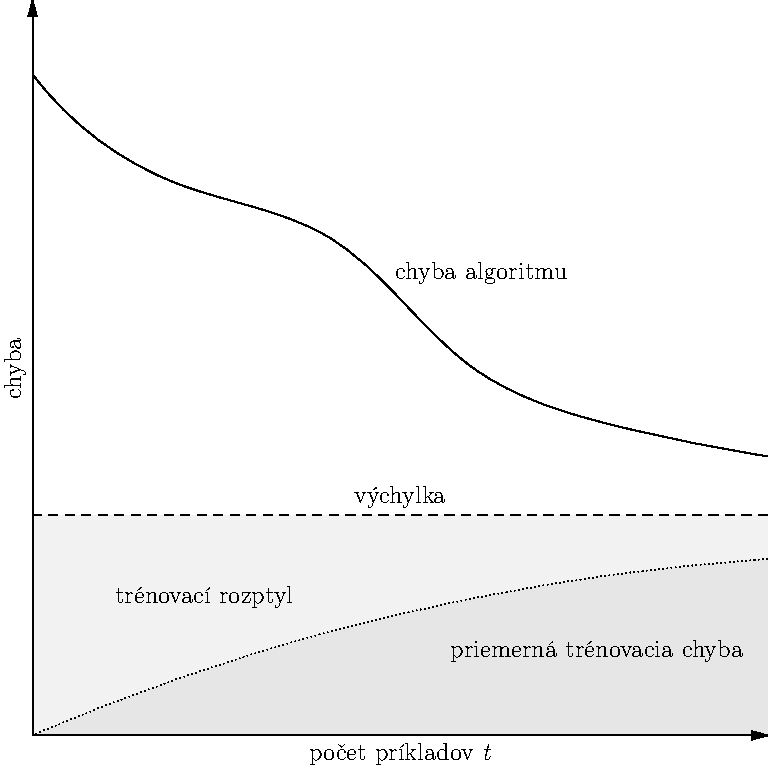
\includegraphics[scale=0.8]{obrazky/krivky1.pdf}
  \caption{Závislosť chyby algoritmu od počtu trénovacích príkladov $t$.}
  \label{img:train}
\end{figure}

\begin{figure}
  \centering
  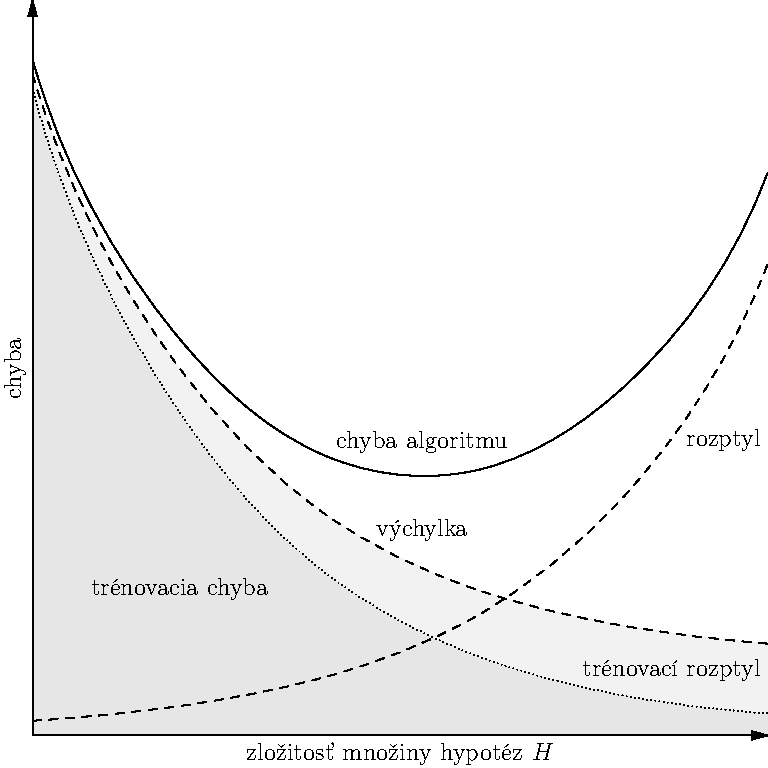
\includegraphics[scale=0.8]{obrazky/krivky2.pdf}
  \caption{Závislosť chyby algoritmu od zložitosti množiny hypotéz $H$.}
  \label{img:hypo}
\end{figure}




\section{Podučenie/preučenie}

Ak máme fixné trénovacie dáta $T$, pri voľbe množiny hypotéz $H$ sa snažíme
nájsť kompromis medzi malým rozptylom a malou výchylkou. Zložité $H$
bude mať malú výchylku ale veľký rozptyl, čo vedie k tzv. \emph{preučeniu}
(angl. \emph{overfitting}). Jednoduché $H$ bude mať malý rozptyl, ale
veľkú výchylku, tzv. \emph{podučenie} (angl. \emph{underfitting}).

Na obrázku \ref{img:fitting} ilustrujeme oba koncepty. Úlohou je modelovať
kvadratickú funkciu, ku ktorej sme pridali malé množstvo šumu. Rozdelenie
$P$ teda vracia nejaké $x$ (napríklad z intervalu $\langle 0, 10 \rangle$)
a $y = x^2 + \varepsilon$, kde $\varepsilon$ je zvolené náhodne z intervalu
$\langle -1, 1 \rangle$. Ak za množinu hypotéz zvolíme lineárne funkcie,
vďaka ich jednoduchosti už pri malých trénovacích množinách bude trénovacia
chyba blízko očakávanej testovacej chyby (nízky rozptyl). Za to ale budú
všetky chyby vysoké (vysoká výchylka). Ak za množinu hypotéz zvolíme polynómy
nejakého vysokého stupňa, ľahko nájdeme polynóm prechádzajúci cez trénovacie
dáta (nízka trénovacia chyba), avšak mimo nich bude dávať výsledky úplne mimo
(vysoká testovacia chyba, a teda vysoký rozptyl).

\begin{figure}
  \centering
  \begin{subfigure}[b]{0.3\linewidth}
    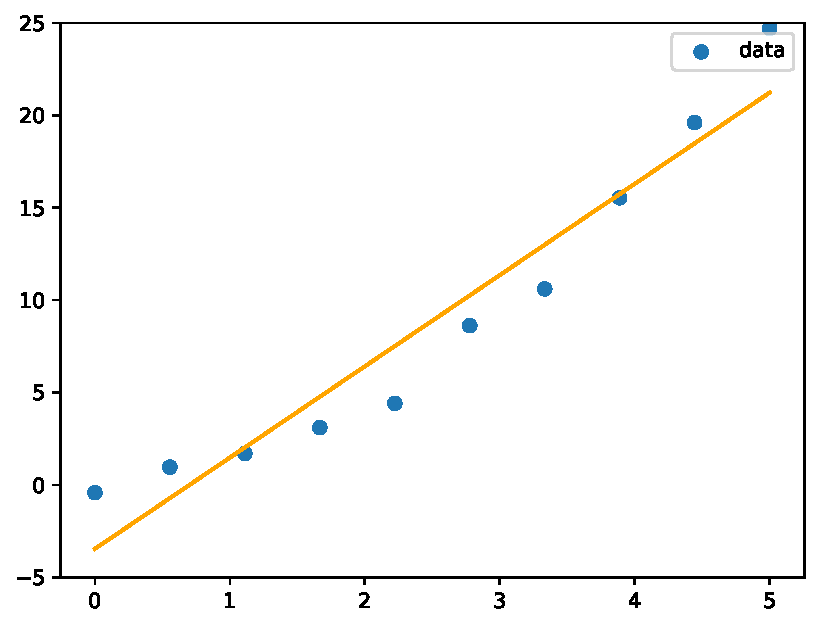
\includegraphics[width=\linewidth]{obrazky/fitting1.pdf}
  \end{subfigure}
  ~
  \begin{subfigure}[b]{0.3\textwidth}
    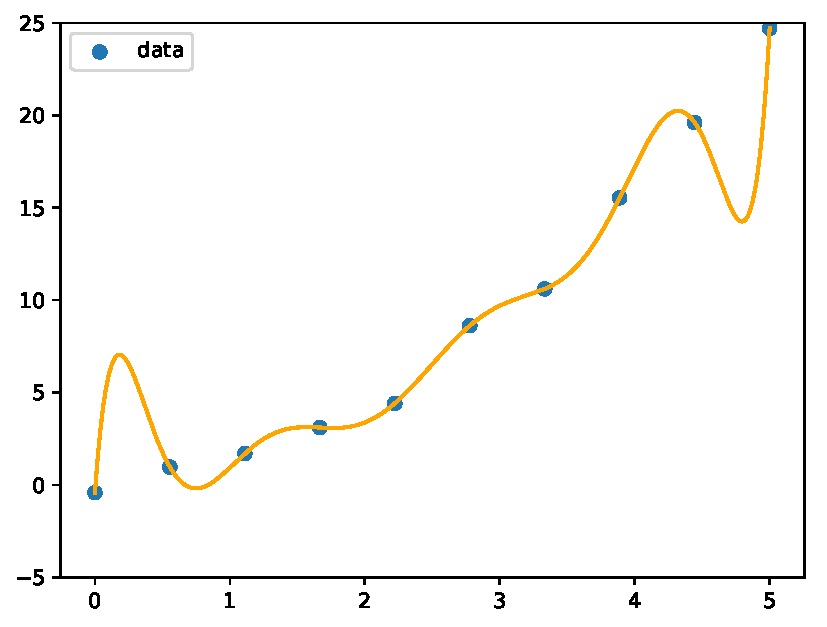
\includegraphics[width=\linewidth]{obrazky/fitting9.pdf}
  \end{subfigure}
  ~
  \begin{subfigure}[b]{0.3\textwidth}
    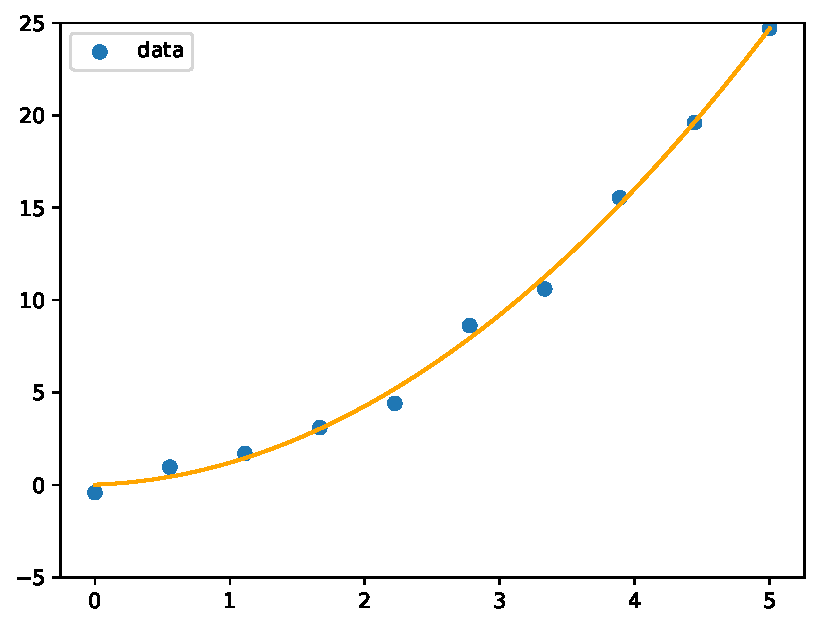
\includegraphics[width=\linewidth]{obrazky/fitting2.pdf}
  \end{subfigure}
  \caption{Podučenie, preučenie, akurát.}
  \label{img:fitting}
\end{figure}



\subsection{Regularizácia}

Predstavme si, že máme na výber z viacerých množín hypotéz $H_1, H_2, \ldots$,
čím ďalej tým zložitejších. Teda $H_1 \subseteq H_2 \subseteq H_3 \subseteq \ldots$.
Ak by sme si graficky znázornili testovacie a trénovacie chyby najlepších
hypotéz z jednotlivých množín, vyzeralo by to zhruba ako na obrázku
\ref{img:multimodels}.

\begin{figure}
  \centering
  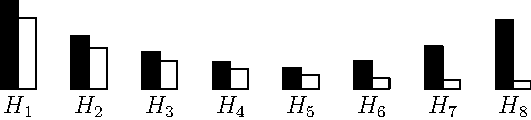
\includegraphics[scale=1]{obrazky/multimodels.pdf}
  \caption{Testovacie (čierne) a trénovacie (biele) chyby v čím ďalej,
    tým zložitejších množinách hypotéz $H$.}
  \label{img:multimodels}
\end{figure}

Z ktorej množiny hypotéz chceme vybrať? Pri trénovaní sa snažíme nájsť
hypotézu $h$, ktorá minimalizuje chybu na trénovacích dátach. Táto
chyba sa ale od očakávanej testovacej chyby líši zhruba
o $\rozptyl + \rozptylT$ (v očakávanom prípade).

V prístupe zvanom \emph{regularizácia} do minimalizovaného výrazu umelo
pridáme \emph{pokutu}, ktorá aproximuje $\rozptyl + \rozptylT$. Tento člen
označíme $\Lambda(h)$. Z čím zložitejšej množiny hypotéza $h$ je, tým
väčšia bude pokuta. Výstupom algoritmu potom je
$$\hat{h}_T = \argmin_{h \in H_1 \cup H_2 \cup \ldots} \left( \Err_T(h) + \Lambda(h) \right).$$

Uvedomme si, že vrámci jednej množiny $H_i$ ostáva ako najlepšia
hypotéza stále tá istá, ako pred zavedením pokuty. V jednej množine
sú totiž všetky hypotézy penalizované rovnako, nerobí to teda rozdiel.
Penalizácia nám ale umožňuje ``férovejšie'' porovnávať hypotézy z rôznych
množín, nakoľko bez pokuty by na tom boli (neprávom) lepšie
zložitejšie hypotézy.

Množiny $H_i$ nemusia byť explicitné, môžu byť implicitne skryté v tom,
aký tvar má výraz $\Lambda(h)$. Do jednej množiny patria tie hypotézy,
ktoré majú rovnakú penalizáciu.

Vo všetkých prípadoch je pokuta parametrizovaná reálnym
parametrom $\lambda$ hovoriacim, ako veľké pokuty chceme udeľovať.
Veľké $\lambda$ (v porovnaní s trénovacou chybou) nám hovorí, že sa
snažíme hlavne dosiahnuť jednoduché hypotézy; s malým $\lambda$ zas
kladieme dôraz na hypotézy s menšou trénovacou chybou.

Uvedieme si niekoľko príkladov výrazov, ktoré sú bežne používané ako
pokuta. Budeme predpokladať, že celá množina hypotéz, z ktorej vyberáme
(tj. $H_1 \cup H_2 \cup \ldots$) je množina lineárnych funkcii
$\R^n \to \R$. Hypotézy majú teda tvar
$$h(x) = a_1x_1 + a_2x_2 + \ldots + a_nx_n.$$
\begin{itemize}
  \item $L_2$ regularizácia (známa aj ako \emph{ridge regression}).
    $$ \Lambda(h) = \lambda \cdot \norm{(a_1, a_2, \ldots, a_n)}^2 = \lambda \cdot (a_1^2 + a_2^2 + \ldots + a_n^2) $$
    Táto pokuta ``tlačí'' váhy nepotrebných atribútov do nuly, pričom
    väčšie váhy tlačí viac. Takže čím dôležitejší atribút, tým väčšiu
    váhu si môže dovoliť mať.
  \item $L_1$ regularizácia (známa aj ako \emph{lasso}).
    $$ \Lambda(h) = \lambda \cdot (|a_1| + |a_2| + \ldots + |a_n|) $$
    Opäť ``tlačíme'' nepotrebné atribúty do nuly, pričom ale všetky
    váhy tlačíme rovnako. To nám vie vynulovať nepotrebné atribúty,
    čo nám vie znížiť výpočtové nároky: nemusíme pri výpočte uvažovať
    tie členy, ktoré majú nulový koeficient.
\end{itemize}



\subsection{Holdout testing}

V tomto prístupe si rozdelíme dostupné dáta na dve časti:
trénovaciu množinu a \emph{validačnú množinu}. Pomocou validačnej
množiny budeme odhadovať testovacie chyby pre jednotlivé množiny
hypotéz, na základe ktorých zistíme, ktorá množina hypotéz je
pre náš problém najvhodnejšia. Konkrétnejšie:
\begin{enumerate}
  \item Trénovaciu množinu použijeme na natrénovanie hypotéz
    z jednotlivých množín.
  \item \label{holdout:step2} Ako odhad testovacej chyby jednotlivých
    hypotéz použijeme ich chybu na validačnej množine. Podľa týchto
    odhadov zistíme, ktorá množina hypotéz je pre náš problém najvhodnejšia.
  \item Použijeme všetky dáta, ktoré máme k dispozícii (tj. z trénovacej
    aj validačnej množiny), na natrénovanie najlepšej možnej hypotézy.
    Berieme samozrejme do úvahy iba hypotézy z tej množiny hypotéz, ktorú
    sme identifikovali ako najvhodnejšiu. Výsledná hypotéza je výstupom
    algoritmu.
\end{enumerate}
 
V kroku \ref{holdout:step2} je dôležité, aby bola validačná
množina nezávislá od trénovacej. Prečo je to dôležité? Môžeme uvažovať
extrémny prípad, keď je validačná množina totožná s trénovacou. Potom
ale ako náš ``odhad'' dostaneme trénovaciu chybu, ktorá rozhodne nie
je dobrým odhadom testovacej chyby. Nezávislosť nám teda zaručuje, že
odhad získaný na validačnej množine je dobrý.

\emph{$k$-fold evaluation.} Pri holdout testovaní je dôležité mať
dobrý odhad testovacej chyby pre jednotlivé množiny hypotéz. Dát ale
môže byť málo, a v takom prípade môže byť odhad nestabilný/nepresný.
Môžeme ale experiment zopakovať niekoľkokrát: v každej iterácii teda
zvolíme inú trénovaciu a inú validačnú množinu, a dostaneme iný odhad
testovacej chyby. Keď tieto odhady spriemerujeme, dostaneme oveľa
presnejší odhad, ako keby sme vykonali iba jednu iteráciu.
V tomto konkrétnom prístupe je $k$ iterácii, a množiny sa volia
nasledovne: všetky dáta sa rozdelia na $k$ zhruba rovnako veľkých
a navzájom nezávislých množín $K_1, K_2, \ldots, K_k$. Následne,
v iterácii $i$ sa ako validačné dáta použije množina $K_i$. Všetko
ostatné budú trénovacie dáta.

\emph{Leave-one-out.} Ak chceme zmerať testovaciu chybu
výstupnej hypotézy, musíme si na to rezervovať ďalšiu časť dát:
\emph{testovaciu množinu}. Tú nepoužívame ani pri trénovaní, ani
pri validácii. Iba úplne na konci celého procesu na nej vypočítame
chybu výslednej hypotézy.




\section{Cvičenia}

V nasledujúcich dvoch cvičeniach môžete predpokladať, že trénovací
algoritmus vždy vráti nejakú funkciu (nemusí byť len jedna)
s minimálnou chybou na trénovacích dátach.

\begin{exercise}
  Je rozumné predpokladať, že s väčším množstvom trénovacích dát sa nám
  bude testovacia chyba zmenšovať. Sú ale zostrojiteľné situácie, kedy
  tomu tak nie je. Nájdite jednu takú situáciu.
  
  Konkrétne, nájdite takú množinu hypotéz $H$ funkcii $\R^n \to \R$
  a rozdelenie $P$, pre ktoré sa bude $\Err(\hat{h}_T)$ so zvyšujúcim
  sa počtom trénovacích chýb \emph{zvyšovať}. Na množinu hypotéz je
  kladená jedna podmienka: pre každú možnú trénovaciu množinu $T$
  musí existovať hypotéza v $H$, ktorá minimalizuje trénovaciu chybu.
  (Teda vždy musí existovať minimum, môže ich byť ale viac. Pre všeobecné
  $H$ vieme povedať iba to, že existuje infimum.)
\end{exercise}

\begin{exercise}
  Za určitých podmienok ale skutočne platí, že viac trénovacích dát
  nám vo veľkom merítku neuškodí. Nech množina hypotéz $H$ je konečná
  a všetky jej funkcie ($\R^n \to \R$) sú ohraničené. Dokážte, že
  pre $t \to \infty$ sa bude OTeCh hypotézy $\hat{h}_T$ blížiť k
  OTeCh najlepšej možnej hypotézy $h^\star$. Inak zapísané, dokážte
  $$\lim_{t \to \infty} \E_T \left[ \Err(\hat{h}_T) - \Err(h^\star) \right] = 0.$$
\end{exercise}

\begin{comment}
\begin{exercise}
  Dokážte korektnosť druhého technického kroku, v odvodení rozkladu
  výchylky na trénovací rozptyl a očakávanú trénovaciu chybu. Konkrétnejšie,
  dokážte
  $$ \E_T \left[ \E_{x_i, y_i} \left[ (h^\star(x_i) - \hat{h}(x_i)) \cdot (\hat{h}(x_i) - y_i) \right] \right] = 0. $$
  Predpoklady kladené na množinu hypotéz sú rovnaké: musí byť uzavretá
  na lineárne kombinácie a na limity.
\end{exercise}
\end{comment}

\begin{exercise}
  Jednou výhodou $L_2$ regularizácie oproti $L_1$ regularizácie je, že
  sa ľahšie minimalizuje výsledný výraz. Ako príklad uvedieme lineárnu
  regresiu. V nej je hypotéza parametrizovaná stĺpcovým vektorom
  $\theta = (\theta_1, \ldots, \theta_n)^T$. Výstupom pre vstup
  $x = (x_1, \ldots, x_n)$ je $x \cdot \theta$. 
  
  Označme $X$ maticu, ktorej riadkami sú vstupy jednotlivých trénovacích
  príkladov. Ďalej nech $y$ je stĺpcový vektor cieľových výstupov na
  jednotlivých príkladoch. Je známe, že optimálnymi parametrami
  lineárnej hypotézy je taký stĺpcový vektor $\theta$, ktorý je riešením
  rovnice
  $$X^T X \cdot \theta = X^T y.$$
  Dokáže, že keď k minimalizovanej hodnote pridáme pokutu vo forme
  $\lambda \cdot \norm{\theta}^2$, tak sa optimálnymi parametrami stane
  $\theta$ riešiaca rovnicu
  $$(X^T X + \lambda I) \cdot \theta = X^T y.$$
  Rozmyslite si tiež, že takéto explicitné vyjadrenie nie je možné
  priamočiaro získať pre $L_1$ regularizáciu.
\end{exercise}




\section{Appendix: iný kompromis medzi inou výchylkou a iným rozptylom}

V literatúre pod názvom \emph{bias-variance tradeoff} vystupuje odlišný
výsledok, ako vyššie spomenutý bias-complexity tradeoff. Uvádzame ho,
pretože sa často zamieňajú a je v tom zmätok. Pokúsime sa vyjasniť, kde
sú rozdiely medzi týmito dvomi výsledkami.

\begin{theorem}
  Zamerajme sa na jeden konkrétny vstup $x$, a merajme chybu výslednej
  hypotézy $\hat{h}_T$ iba na tomto vstupe. (Stále ale môžeme dostať
  rôzne $y$.) Na meranie chyby použijeme kvadratickú odchýlku. Označme
  očakávanú hodnotu tejto chyby (cez všetky možné trénovacie
  množiny $T$ a výstupy $y$) ako $\Err_{|x=x}(L)$. Tvrdíme, že
  sa dá vyjadriť nasledovne:
  $$
    \Err_{|x=x}(L)
      = \underbrace{\Var_T \left( \hat{h}_T(x) \right)}_{\text{\normalfont rozptyl}}
      + \underbrace{\left( \E_T \left[ \hat{h}_T(x) \right] - h^\square(x) \right)^2}_{\text{\normalfont výchylka}^2}
      + \underbrace{\E_y \left[ \varepsilon^2 \right]}_{\text{\normalfont šum}},
  $$
  kde $\varepsilon := y - h^\square(x)$.
\end{theorem}

Zastavme sa najprv nad tým, ako toto tvrdenie interpretovať. Pre každú
možnú vzorku trénovacích dát $T$ dostaneme nejakú inú hypotézu $\hat{h}_T$.
Rozptyl je nízky práve vtedy, keď budú všetky tieto hypotézy dávať
podobné výsledky. Ak je vysoký, znamená to, že výsledná hypotéza je
veľmi citlivá na trénovacie dáta; oplatí sa preto zväčšiť ich množstvo.
(Ak chceme byť veľmi skeptický, nič nezaručuje, že zväčšením trénovacej
množiny sa rozptyl zníži. Možno existuje iný dôvod, kvôli ktorému je
vysoký; takmer určite sa dajú skonštruovať takéto umelé protipríklady.)

Keď už uvažujeme všetky možné výsledné hypotézy $\hat{h}_T$, môžme sa
pozrieť na to, aký je ich ``priemerný odhad'': ak by sme spriemerovali
všetky ich výsledky, čo by sme dostali? Presne $\E_T [ \hat{h}_T(x) ]$;
výchylka-na-druhú potom meria, o koľko sa takáto priemerná hypotéza líši od
najlepšej možnej funkcie $h^\square$. Ak je výchylka vysoká ale variancia
nízka, znamená to, že takmer všetky $\hat{h}_T$ majú problém na vstupe $x$,
treba teda zvážiť voľbu zložitejšej množiny hypotéz.

Nakoniec, šum zodpovedá ireducibilnej chybe, ktorú bude mať každá hypotéza.
Je to v dôsledku toho, že jednému $x$ môže pripadať viacero rôznych $y$.
Presne túto chybu nadobúda najlepšia hypotéza-funkcia $h^\square$ (pre
ktorú sú rozptyl aj výchylka-na-druhú nulové).

\begin{proof}
  Upravujme pôvodný výraz.
  \begin{align}
    \Err_{|x=x}(L)
      &= \E_{T, y} \left[ (\hat{h}_T(x) - y)^2 \right] \\
      &= \E_{T, y} \left[ ((\hat{h}_T(x) - h^\square(x)) - \varepsilon)^2 \right] \\
      &= \E_{T, y} \left[ (\hat{h}_T(x) - h^\square(x))^2 + \varepsilon^2 - 2 \cdot \varepsilon \cdot (\hat{h}_T(x) - h^\square(x)) \right] \label{align:roznasob} \\
      &= \E_T \left[ (\hat{h}_T(x) - h^\square(x))^2 \right] + \E_y \left[ \varepsilon^2 \right] - \E_{T, y} \left[ 2 \cdot \varepsilon \cdot (\hat{h}_T(x) - h^\square(x)) \right] \label{align:linearita} \\
      &= \E_T \left[ (\hat{h}_T(x) - h^\square(x))^2 \right] + \E_y \left[ \varepsilon^2 \right] - 2 \cdot \E_y \left[ \varepsilon \right] \cdot \E_T \left[ (\hat{h}_T(x) - h^\square(x)) \right] \label{align:sucin_nezavislych} \\
      &= \E_T \left[ (\hat{h}_T(x) - h^\square(x))^2 \right] + \E_y \left[ \varepsilon^2 \right] \label{align:epsilon_nula}
  \end{align}
  Výraz sme upravili, potom v kroku \ref{align:roznasob} roznásobili a v kroku
  \ref{align:linearita} využili linearitu strednej hodnoty.
  Ďalej v kroku \ref{align:sucin_nezavislych} sme využili, že
  stredná hodnota súčinu nezávislých premenných je súčinom stredných
  hodnôt tých premenných. Nakoniec v kroku \ref{align:epsilon_nula}
  využívame $\E \left[ \varepsilon \right] = 0$. Zamerajme sa ďalej na prvý sčítanec.
  \begin{align}
    &= \E_T \left[ (\hat{h}_T(x) - h^\square(x))^2 \right] \\
    &= \E_T \left[ \hat{h}_T(x)^2 + h^\square(x)^2 - 2 \cdot \hat{h}_T(x) \cdot h^\square(x) \right] \label{align:roznasob2} \\
    &= \E_T \left[ \hat{h}_T(x)^2 \right] + \E_T \left[ h^\square(x)^2 \right] - \E_T \left[ 2 \cdot \hat{h}_T(x) \cdot h^\square(x) \right] \label{align:linearita2} \\
    &= \left( \Var_T \left( \hat{h}_T(x) \right) + \E_T \left[ \hat{h}_T(x) \right]^2 \right) + \left( \Var_T \left( h^\square(x) \right) + \E_T \left[ h^\square(x) \right]^2 \right) - \E_T \left[ 2 \cdot \hat{h}_T(x) \cdot h^\square(x) \right] \label{align:var_alt} \\
  \end{align}
  V kroku \ref{align:roznasob2} sme výraz roznásobili a potom v kroku
  \ref{align:linearita2} využili linearitu strednej hodnoty. V poslednom
  kroku (\ref{align:var_alt}) sme využili vzťah $\Var(a) = \E \left[ a^2 \right] - \E \left[ a \right]^2$.
  Pokračujme ďalej v úpravách.
  \begin{align}
    &= \left( \Var_T \left( \hat{h}_T(x) \right) + \E_T \left[ \hat{h}_T(x) \right]^2 \right) + h^\square(x)^2 - 2 \cdot \E_T \left[ \hat{h}_T(x)  \right] \cdot h^\square(x) \label{align:square_const} \\
    &= \Var_T \left( \hat{h}_T(x) \right) + \left( \E_T \left[ \hat{h}_T(x) \right]^2 + h^\square(x)^2 - 2 \cdot \E_T \left[ \hat{h}_T(x)  \right] \cdot h^\square(x) \right) \\
    &= \Var_T \left( \hat{h}_T(x) \right) + \left( \E_T \left[ \hat{h}_T(x) \right] - h^\square(x) \right)^2
  \end{align}
  V kroku \ref{align:square_const} sme využili, že $x$ je vopred dané,
  a teda $h^\square(x)$ je konštanta. Má teda nulový rozptyl a jeho
  stredná hodnota je identická s jeho hodnotou. Ďalej sme už len
  upravovali. Keď to celé dáme do jednej rovnice, dostaneme
  $$
    \Err_{|x=x}(L)
      = \underbrace{\Var_T \left( \hat{h}_T(x) \right)}_{\text{\normalfont rozptyl}}
      + \underbrace{\left( \E_T \left[ \hat{h}_T(x) \right] - h^\square(x) \right)^2}_{\text{\normalfont výchylka}^2}
      + \underbrace{\E_y \left[ \varepsilon^2 \right]}_{\text{\normalfont šum}}.
  $$
\end{proof}
